\documentclass[10pt]{beamer}

\usetheme{default}

\usepackage[utf8]{inputenc}
\usepackage[russian]{babel}
\usepackage[OT1]{fontenc}
\usepackage{amsmath}
\usepackage{amsfonts}
\usepackage{amssymb}
\usepackage{graphicx}
\usepackage{etoolbox}
\usepackage{caption}
\usepackage{subcaption}
\usepackage{pifont}
\usepackage{xcolor}
\usepackage{framed}
\definecolor{shadecolor}{cmyk}{0,0,0,1}

\makeatletter

\setbeamercolor{title}{fg=white}
\setbeamercolor{frametitle}{fg=black}
\setbeamerfont*{title}{family=\sffamily,size=\LARGE}

\setbeamerfont{page number in head/foot}{size=\scriptsize}
\setbeamertemplate{footline}[frame number]
\let\otp\titlepage
\renewcommand{\titlepage}{\otp\addtocounter{framenumber}{-1}}

\setbeamertemplate{background canvas}{%
	\ifnumequal{\c@framenumber}{0}{%
      
\includegraphics[width=\paperwidth,height=\paperheight]{images/cover.png}
   }{%
      \ifnumequal{\c@framenumber}{\inserttotalframenumber}{
         
\includegraphics[width=\paperwidth,height=\paperheight]{images/back.png}
      }{%
         % Other frames
      }%
   }%
}

\makeatother

\beamertemplatenavigationsymbolsempty

\author{Ксения Стройкова}
\title{\newline \newline \newline Анализ графов в социальных медиа}

\begin{document}

\begin{frame}[plain]
\titlepage
\end{frame}

\begin{frame}{Python in Twitter}

\begin{center}
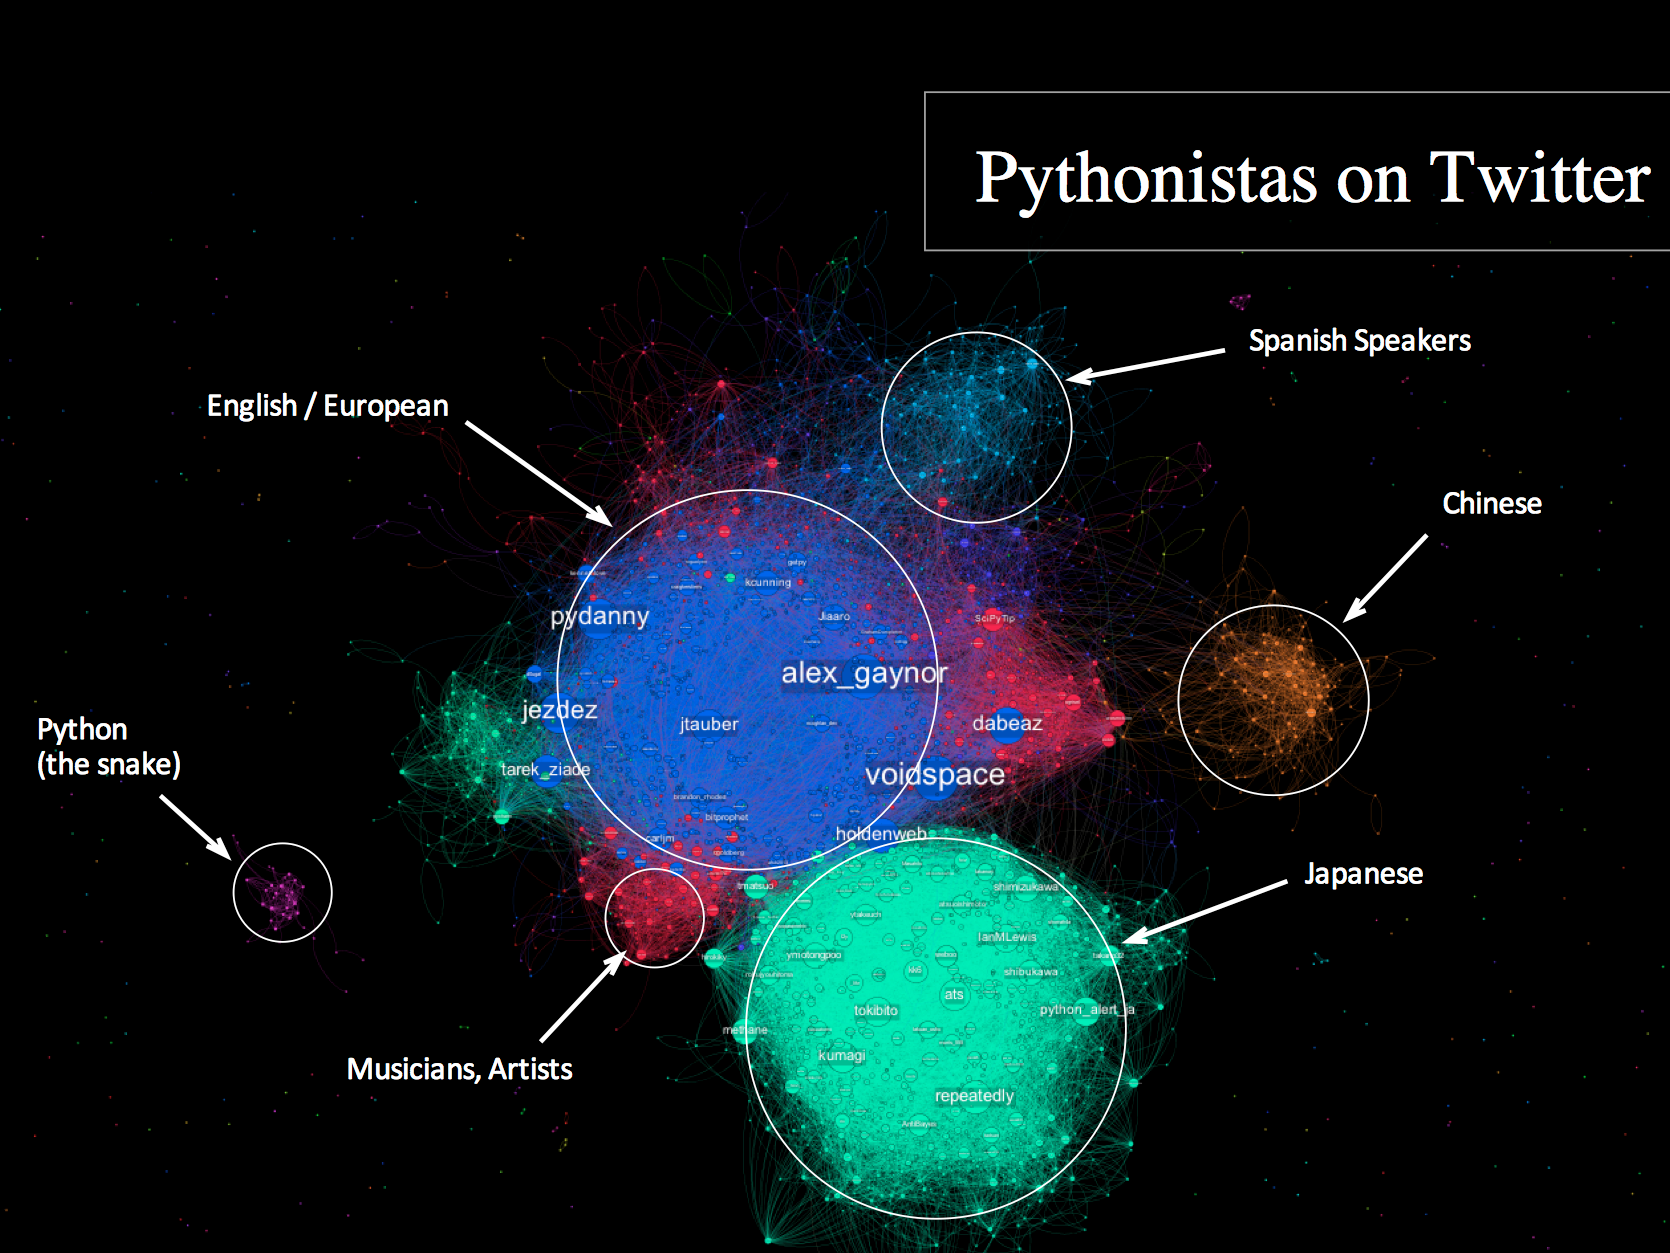
\includegraphics[scale=0.18]{images/python.png}
\end{center}

\end{frame}

\begin{frame}{Содержание}
\tableofcontents
\end{frame}

% =======================
\section{Постановка задачи}
% =======================

\begin{frame}{Задачи анализа социальных графов}

{\small
\begin{enumerate}
\item Социальный поиск - поиск объектов по социальным связям
\item Генерация рекомендаций - друзей или контента
\item Выявление настоящих связей
\item Лидеры мнений
\item Поиск сообществ
\item Уточнение интересов
\item Распространение новостей о событиях
\end{enumerate}
}

\end{frame}

\begin{frame}{Warface}

\begin{block}{Задачи}
\begin{itemize}
\item Поиск игроков, которые могут покинуть игру при уходе данного игрока
\item Оценка общей стоимости ухода такого игрока
\item Социальные рекомендации для игроков
\end{itemize}
\end{block}

\begin{block}{Особенности}
\begin{itemize}
\item Неявные связи
\item Сессионность игры
\item Данные меняются со временем
\end{itemize}
\end{block}

\begin{block}{Ближайшие цели}
\begin{itemize}
\item Поиск сообществ
\item Оценка влияния игрока на других
\end{itemize}
\end{block}

\end{frame}

% =======================
\section{Исходные данные}
% =======================


\begin{frame}{Исходные данные}

\begin{itemize}
\item Лог сессий игроков
\item Лог сообщений игроков
\item Общий лог событий (клановые события, отношения друзей)
\item Лог покупок
\end{itemize}


\end{frame}

% =======================
\section{Метрики в графе}
% =======================

\begin{frame}{Граф}
\[
G = \left(V, E\right)
\]
G- граф
V - вершины
E - ребра
\begin{center}
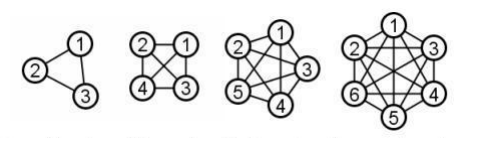
\includegraphics[scale=0.5]{images/1.png}
\end{center}

\end{frame}

\begin{frame}{Метрики в графе}

\begin{block}{Degree}
\[
C_d\left(v_i\right) = k_i = number\ of\ neighbors
\]
\end{block}

\begin{block}{Betweenness}
\[
C_b\left(v\right) = \sum\frac{\sigma_{st}(v)}{\sigma_{st}} = 
shortest\ paths / all\ paths
\]
\end{block}
	
\begin{block}{Closeness}
\[
C_c\left(v\right) = \frac{1}{\sum d(y,x)} = distance\ to\ other\ nodes
\]
\end{block}

\end{frame}

% =======================
\section{Поиск сообществ}
% =======================

\begin{frame}{Modularity}



\begin{block}{Метрика, оценивающая насколько внутренних связей в сообществе больше, чем внешних}
\[
Q = \frac{1}{2m} \sum\left(A_{ij} - \frac{k_i k_j}{2m}\right)\delta\left(c_i,c_j\right)
\]
\end{block}

\begin{itemize}
\item $A_ij$ - общее количество связей внутри сообщества
\item $\frac{k_i k_j}{2m}$ - ожидаемое количество ребер между i и j, если ребра распределены случайно
\item m - количество ребер в графе
\item $\delta = 1$, если вершины в одном и том же сообществе
\item c - сообщество вершины
\item k - degree вершины
\end{itemize}

\end{frame}


\begin{frame}{Поиск сообществ}

\begin{itemize}
\item Максимизация modularity - метрики качества структуры сообществ
\item Иерархическая кластеризация
\item Поиск за $n\log n$
\end{itemize}

\end{frame}


\end{document}